\documentclass[10pt]{article}

% Minimal packages for fast compile
\usepackage{times}
\usepackage[utf8]{inputenc}
\usepackage[T1]{fontenc}
\usepackage[a4paper,margin=2cm]{geometry}
\usepackage{titlesec}
\usepackage{graphicx}
\usepackage{booktabs}
\usepackage{float}
\usepackage[section]{placeins}
\usepackage{setspace}

% Section title styles
\titleformat{\section}{\bfseries\fontsize{12}{14}\selectfont}{\thesection.}{0.5em}{}
\titleformat{\subsection}{\bfseries\fontsize{11}{13}\selectfont}{\thesubsection.}{0.5em}{}

% Custom title page
\begin{document}

\begin{titlepage}
\centering
\vspace*{2cm}

\includegraphics[width=0.3\textwidth]{image.png}
\vspace{1cm}

{\Huge\bfseries Status Report\par}
\vspace{2cm}

\begin{flushleft}
\textbf{Name of submission:} Status report 2\\[0.5em]
\textbf{Group name:} Testbench for Bit-Serial RISC-V processor in SoI for Venus\\[0.5em]
\textbf{Date:} 2025/12/02\\[0.5em]
\textbf{Organization:} KTH\\[1.5em]
\textbf{Authors:}\\[0.5em]
\begin{center}
\begin{tabular}{p{5cm}p{6cm}}
\toprule
\textbf{Name} & \textbf{Email} \\
\midrule
Chinmay Purandare & \texttt{chinmayp@kth.se} \\
Lorenzo Parata & \texttt{parata@ug.kth.se} \\
Chongnan Wang & \texttt{chongnan@kth.se} \\
Xiaotian Jiang & \texttt{xjia@kth.se} \\
Xinxin Qin & \texttt{xinxinq@kth.se} \\
Paul Martin & \texttt{paulmart@kth.se} \\
\bottomrule
\end{tabular}
\end{center}
\vspace{1em}
\end{flushleft}

\vfill
\begin{flushright}
\textbf{Department of Electronics}\\
KTH Royal Institute of Technology\\
Stockholm, Sweden
\end{flushright}
\end{titlepage}

% Table of Contents on separate page
\clearpage
\tableofcontents
\thispagestyle{plain}
\clearpage

% Start main content
\section{General description of status} 
• What has happened since the last report?\\
• What is the status?


\section{Resource Status}
• How much in terms of resources has the project consumed and how much has been
delivered?\\
• (In industrial projects, the economic status is reported as well)


\section{Problems / Action plan}
• State the problems the sponsor and steering committee need to be aware of, and
proposals for action

\newpage
\section{Risks / Action plan}
Since the last risk analysis, the team has continued to monitor risks. Indeed, several risks have evolved along the development. That is why it is importante de do an updated section where we are going to present you the current situation.

\subsection{Follow-up of Risk Analysis}
During the last few springs, risk management has proven to be useful. Indeed, some of the risks we previously identified did occur but were handled with success.
\begin{itemize}
    \item \textbf{Verification coverage} - Testbench may not provide full functional testing, so we decided to use CoreMark for that. It is a standard benchmark developed to measure the performance of a processor's core. It’s a perfect fit for us because it provides a simple and quick way to compare different CPUs, especially those found in embedded systems.
    \item \textbf{Coordination and availability} - As we expected, the different schedules of the team members create delays in communication. We manage this by writing reports on every meeting and by adapting the date of meetings accordingly to the team's availability.
    \item \textbf{Integration timeline underestimation} - fSystem-level testing has taken longer than expected. However, we are still on time thanks to the allocated buffer time we have set at the start of the project.
    \item \textbf{Extreme Environment} - After discussion with our professor, making our FPGA resistant to extreme environments is not a requirement for our project. Indeed, another team will probably in the future work on this aspect by selecting different materials and applying triplication techniques to protect the design from radiation.
\end{itemize}

\subsection{Updated Risk Analysis}
Here is the new version of our risk analysis table and matrix. To simplify, we erased the ones that became insignificant during our previous analysis, that is to say risks 4, 12, 8, 13, 9. We have also updated a few risks and added new ones.
\begin{table}[h!]
\centering
\begin{tabular}{|c|p{2.35cm}|p{4.1cm}|c|c|c|p{4.3cm}|p{1.17cm}|c|}
\hline
\textbf{ID} & \textbf{Risk} & \textbf{Description} & \textbf{P} & \textbf{C} & \textbf{R} & \textbf{Suggested Action} & \textbf{Follow-up Date} & \textbf{Trend} \\
\hline
1 & Hardware complexity & Two processor models on separate FPGAs increase design and debugging effort. & 3 & 4 & 12 & Start with single-FPGA setup, define early comm. protocols. & 31 Oct & $\downarrow$ \\
\hline
2 & Multi-FPGA system complexity & Communication and timing between boards difficult to synchronize. & 4 & 4 & 16 & Test modules separately, simulate before hardware link. & 31 Oct & $\rightarrow$ \\
\hline
3 & Extreme environment & SoI may not survive Venus-like temperatures. & 2 & 5 & 10 & Study environmental limits; keep simulation-level validation. & 28 Nov & $\downarrow$ \\
\hline
5 & Performance gap & Bit-serial version may not reach required speed. & 4 & 3 & 12 & Define realistic targets, compare to parallel baseline. & 31 Oct & $\rightarrow$ \\
\hline
6 & Verification coverage & Testbench may not provide full functional testing. & 3 & 5 & 15 & Add random/stress test patterns; document coverage. & 28 Nov & $\downarrow$ \\
\hline
7 & Specialized toolchain dependency & ProGram compiler unstable or limited. & 3 & 3 & 9 & Validate early, keep VHDL rewrite backup plan. & 24 Oct & $\downarrow$ \\
\hline
10 & Internal conflicts & Potential disagreements between members. & 3 & 4 & 12 & Address through discussion or reassigning tasks. & 31 Oct & $\rightarrow$ \\
\hline
11 & Integration timeline underestimation & System-level testing may take longer than expected. & 5 & 3 & 15 & Allocate buffer time, set MVP milestone. & 31 Oct & $\rightarrow$ \\
\hline
14 & Clock domain and timing inconsistencies & Different clocks between the two FPGAs can cause missed pulses or unreliable data transfers. & 4 & 4 & 16 & Define a clear clocking strategy. Add synchronizers, handshake protocols or even PLL if needed. & 28 Nov & $\uparrow$ \\
\hline
\end{tabular}
\caption{Mini Risk Method Table}
\end{table}

\begin{figure}[h!]
    \centering
    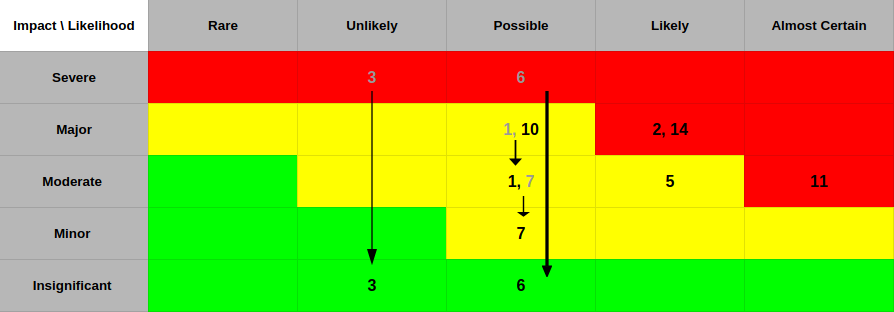
\includegraphics[width=1\textwidth]{risk_matrix_v2.png}
    \caption{Updated Risk Matrix}
\end{figure}

\subsection{Risks to Be Reported}

According to the current risk matrix, 3 risks are currently considered highly critical for the project (in the red zone) and need important attention. 

We have especially Risk 2 – Multi-FPGA System Complexity and Risk 11 – Integration Timeline Underestimation that remain an important concern, as we already talk about in the previous status report.

But we have in addition Risk 14 – Clock Domain and Timing Inconsistencies that is new. During multi-FPGA integration, even small clock differences between the processor board and the testbench board can lead to errors. However, the 2 FPGAs do not share the exact same clock and it might lead to timing drift and signal synchronization issues. To avoid this, it is important to have proper synchronizers and handshake logic. In the worst case scenario, we might even need to implement an PLL.


\section{Project changes from the project plan}
• This is where changes are documented so that they become visual. Changes are
typically: new requirements, changed requirements, changed organization, changed
prerequisites, new documents, etc.


\section{Appendix}
• Updated time plan\\
• Updated resource plan


\end{document}
